\documentclass[usenames,dvipsnames]{beamer}
\usepackage[utf8]{inputenc}
\usepackage{verbatim}
\usetheme{umu}

\usepackage[inline]{enumitem}
\usepackage[labelformat=empty]{caption}
\captionsetup[figure]{font=scriptsize}
\usepackage{siunitx}
\usepackage{xcolor}



%%% Some useful commands
% pdf-friendly newline in links
\newcommand{\pdfnewline}{\texorpdfstring{\newline}{ }} 
% Fill the vertical space in a slide (to put text at the bottom)
\newcommand{\framefill}{\vskip0pt plus 1filll}
\setbeamertemplate{caption}{\raggedright\insertcaption\par}

%%%%%%%%%%%%%%%%%%%%%%%%%%%%%%%%%%%%%%%%%%%%%%%%%%%%%%%%%%%%%%%%%%%%%%%%%%%%%%%%%%%%%
%%%%%%%%%%%%%%%%%%%%%%%%%%%%%%% YOUR PRESENTATION BELOW %%%%%%%%%%%%%%%%%%%%%%%%%%%%%
%%%%%%%%%%%%%%%%%%%%%%%%%%%%%%%%%%%%%%%%%%%%%%%%%%%%%%%%%%%%%%%%%%%%%%%%%%%%%%%%%%%%%
\title{Évolution de la dynamique des galaxies au cours des $10$ derniers milliards d'années avec MUSE/VLT}

\date[\today]{\small\today}
\author[Mercier Wilfried]{
  \textbf{\large{Mercier Wilfried}}}

\begin{document}

\begin{frame}
\titlepage
 \end{frame}
 
\section{Mon parcours}
\begin{frame}{Mon parcours}
	\begin{itemize}[label=$\rhd$]
		\item Lience mention Bien \\ $\rightarrow$ Université de Bordeaux
		\item \textbf{ERASMUS+} (L3) \\ $\rightarrow$ Université de Bristol, Angleterre 
	\end{itemize}
	\vfill
	\begin{itemize}[label=$\rhd$]
		\item M1 mention Très Bien et M2 \\ $\rightarrow$ Observatoire de Paris
	\end{itemize}
	\vfill
	\begin{itemize}[label=$\rhd$]
		\item \textbf{3 stages} de recherche en Astrophysique
	\end{itemize}
	\hspace{20pt} $\cdot$ Laboratoire d'Astrophysique de Bordeaux (L1)\\
	\hspace{20pt} $\cdot$ Institut d'Astrophysique de Paris (M1)\\
	\hspace{20pt} $\cdot$ IRAP (M2)
	
	%logos
	\begin{textblock*}{3cm}(9.5cm, 1.2cm)
		\includegraphics[width=\linewidth]{{graphics/univ_bordeaux}.png}
	\end{textblock*}
	
	\begin{textblock*}{3cm}(9.5cm, 2.5cm)
		\includegraphics[width=\linewidth]{{graphics/univ_Bristol}.jpg}
	\end{textblock*}
	
	\begin{textblock*}{3cm}(9.5cm, 4cm)
		\includegraphics[width=\linewidth]{{graphics/logo_obspm}.png}
	\end{textblock*}

	
	\begin{textblock*}{2cm}(10cm, 7cm)
		\includegraphics[width=\linewidth]{{graphics/iap}.jpg}
	\end{textblock*}
	
	\begin{textblock*}{2cm}(10.1cm, 5.8cm)
		\includegraphics[width=\linewidth]{{graphics/lab}.png}
	\end{textblock*}
	
	\begin{textblock*}{2cm}(8cm, 8.2cm)
		\includegraphics[width=\linewidth]{{graphics/irap_logo}.png}
	\end{textblock*}
	
\end{frame}




\section{Stages Master : M1}
\begin{frame}{Stages Master : M1 (IAP)}
	
	\begin{textblock*}{11cm}(1.8cm, 1.5cm)
		Comment retrouver les \underline{propriétés} des \textbf{amas de galaxies} ?
	\end{textblock*}
	\begin{textblock*}{7cm}(0.5cm, 2.5cm)
		\includegraphics[width=\linewidth]{{graphics/ell2_AMICO}.pdf}
	\end{textblock*}
	
	\begin{textblock*}{6cm}(7.4cm, 5cm)
		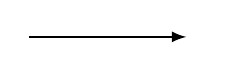
\begin{tikzpicture}[thick]
			\draw [black,   -latex      ] (7,7.0) -- (9,7.0) node [right] {};
		\end{tikzpicture}
	\end{textblock*}
	
	\begin{textblock*}{10cm}(10cm, 4.5cm)
		Taille ? \\ 
		Ellipticité ? \\
		Rotation ?
	\end{textblock*}
	
	\begin{textblock*}{2.5cm}(7.1cm, 3.8cm)
		\centering
		\large \textbf{Code \\
		PROF-CL}
	\end{textblock*}
	
	\begin{textblock*}{11cm}(1.1cm, 8.2cm)
		\centering
		\large En préparation de la future \textbf{mission EUCLID} (2022)
	\end{textblock*}
	
\end{frame}






\section{Stages Master : M2}
\setbeamercolor{background canvas}{bg=black}
\begin{frame}{Stages Master : M2 (IRAP)}
	\framesubtitle{La \textcolor{red}{grande question} en Astrophysique extra-galactique}
	
	\begin{textblock*}{10cm}(1cm,1.66cm)
		\begin{tikzpicture}
			\useasboundingbox (0,-0.05) rectangle(\the\paperwidth,9.2);
			\fill[color=black] (-2,0+1.60) rectangle(\the\paperwidth,0.03+1.70);
	  	\end{tikzpicture}
  	\end{textblock*}
	
	\begin{textblock*}{11cm}(0.5cm,1.66cm)
		\centering
		\includegraphics[width=1.1\linewidth]{{graphics/evolution_gals}.pdf}
  	\end{textblock*}
  	
  	\begin{textblock*}{6cm}(2.5cm, 7.3cm)
		\begin{tikzpicture}[thick]
			\draw [white,   -latex      ] (17,7.0) -- (9,7.0) node [right] {};
		\end{tikzpicture}
	\end{textblock*}
	
	\begin{textblock*}{12cm}(0.4cm, 8cm)
		\centering
		\Large \textbf{\textcolor{red}{Comment expliquer la croissance des galaxies ?}}
	\end{textblock*}

	
\end{frame}







\setbeamercolor{background canvas}{bg=white}
\color{black}

\begin{frame}{Avec des données MUSE}
	\begin{columns}
		\begin{column}{0.45\linewidth}
			\begin{itemize}[label=$\rhd$]
				\item Détection de galaxies\\ \textcolor{blue}{$z = 0.1$} et \textcolor{red}{$z = 6.3$} \\
				
				$\rightarrow$ de \textcolor{blue}{1.2} à \textcolor{red}{$\SI{12.2}{Gyr}$} \\dans le passé
				
				\item très faible masse
			\end{itemize}
			
			\vspace{20pt}
			Sélection d'un \textbf{échantillon} pour modéliser la \textbf{cinématique}:
			\begin{itemize}[label=$\rhd$]
				\item $0.4 \leq z \leq 1.4$
				\item rayon assez grand \\
				$\Rightarrow$ beaucoup de pixels pour la modélisation
			\end{itemize}			
			
		\end{column}
		
		\begin{column}{0.7\linewidth}
			\vspace{-30pt}
			\begin{figure}
				\includegraphics[width=\linewidth]{{graphics/champs_hdfs_bacon}.eps}
			\end{figure}
		\end{column}
	\end{columns}
	
	\begin{textblock*}{10cm}(6.4cm, 8.3cm)
		\footnotesize Galaxies dans l'HDFS avec des redshifts \\ spectroscopiques précis mesurés par MUSE.
	\end{textblock*}
\end{frame}





\begin{frame}{Stages Master : M2 (IRAP)}
	\framesubtitle{MUSE}

	\begin{columns}	
		\begin{column}{0.5\linewidth}
			\begin{figure}
				\vspace{-15pt}
				\centering
				\includegraphics[width=0.9\linewidth]{{graphics/MUSE_tcontini2}.jpg}
				\caption{MUSE instrument. Credit: Contini Thierry (IRAP)}
			\end{figure}
		\end{column}
		\begin{column}{0.6\linewidth}
			\vspace{70pt}		
			\centering
			
\includegraphics[width=0.5\linewidth]{{graphics/VelBefore}.eps}
		\end{column}
	\end{columns}
	
	
	\begin{textblock*}{6cm}(6.5cm, 1.3cm)
		Galaxie observée telle qu'elle était il y a \textbf{6 milliards d'années}
	\end{textblock*}
	
	\begin{textblock*}{6cm}(5.55cm, 3.1cm)
		\Large{Cube 3D}
	\end{textblock*}	
	
	\begin{textblock*}{6cm}(7.3cm, 3.4cm)
		\textbf{+140 km/s}
	\end{textblock*}
	
	\begin{textblock*}{6cm}(10.5cm, 4.6cm)
		\textbf{{\Large -}140 km/s}
	\end{textblock*}
	
	
	%big arrow
	\begin{textblock*}{6cm}(5.5cm, 3.8cm)
		
\begin{tikzpicture}[thick]
			\draw [black,   -latex, line width=3pt     ] (9,7.0) -- (11,7.0) node [right] {};
		\end{tikzpicture}
	\end{textblock*}
	
		%arrow for bad spectrum
	\begin{textblock*}{5cm}(5.1cm, 4.8cm)
		\centering
		\begin{tikzpicture}[thick]
			\draw [black,   -latex      ] (0,7.0) -- (1,9) node [right] {};
		\end{tikzpicture}
	\end{textblock*}
	
	%arrow for medium spectrum
	\begin{textblock*}{5cm}(6.7cm, 4.6cm)
		\centering
		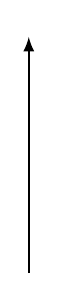
\begin{tikzpicture}[thick]
			\draw [black,   -latex      ] (3,10.0) -- (3,13) node [right] {};
		\end{tikzpicture}
	\end{textblock*}
	
	%arrow for good spectrum
	\begin{textblock*}{5cm}(8cm, 3.8cm)
		\centering
		\begin{tikzpicture}[thick]
			\draw [black,   -latex      ] (4.5,5.0) -- (2,8.5) node [right] {};
		\end{tikzpicture}
	\end{textblock*}
	
		%three spectra
	\begin{textblock*}{6.5cm}(6cm,7cm)
		\centering
		\includegraphics[width=0.25\linewidth]{{graphics/BadSpectrum}.png}
		\hfill
		\includegraphics[width=0.25\linewidth]{{graphics/MediumSpectrum}.png}
		\hfill
		\includegraphics[width=0.25\linewidth]{{graphics/GoodSpectrum}.png}
	\end{textblock*}	
\end{frame}
 




\begin{frame}{Les grandes étapes du stage}
	\begin{textblock*}{11.5cm}(0.1cm, 1.2cm)
		
\includegraphics[width=1.1\linewidth]{{graphics/Schematics}.eps}
	\end{textblock*}
	
	\begin{textblock*}{11cm}(8.6cm, 3cm)
		\textbf{\textcolor{blue}{Morphologie} \\ 
		\textcolor{magenta}{Cinématique} \\ 
		\textcolor{orange}{Analyse des données}}
	\end{textblock*}
	

\end{frame}




\subsection{Fitting a model}
\begin{frame}{Stages Master : M2 (IRAP)}
	\framesubtitle{Modéliser la cinématique des galaxies avec un disque en rotation}
	
	\begin{textblock*}{6cm}(1cm, 1.2cm)
		\centering
		\hspace*{5pt}
		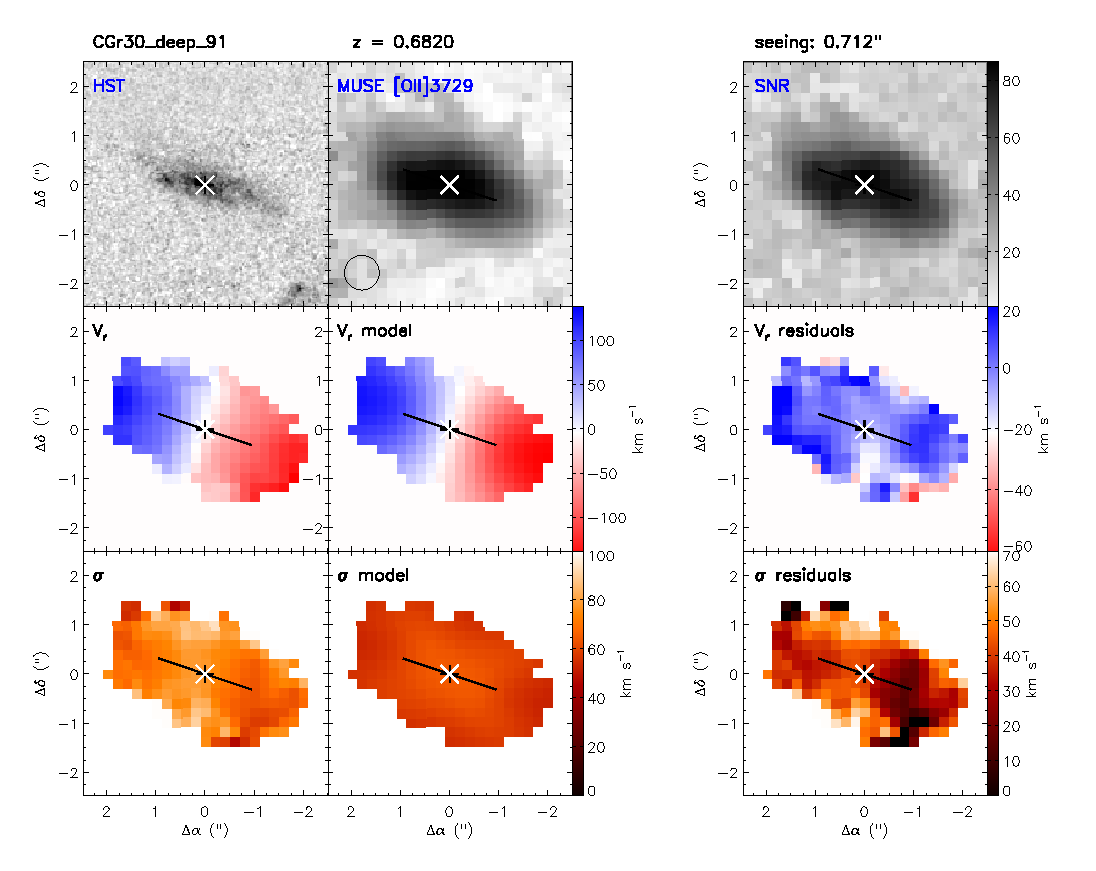
\includegraphics[width=\linewidth]{{graphics/maps_CGr30_deep_91_o2_paper}.eps}
	\end{textblock*}
	
	
	\begin{textblock*}{5cm}(8.2cm, 2.2cm)
		\Large
		Cartes de vitesses
		\begin{enumerate}[label=\alph*.]
			\item \textcolor{OliveGreen}{ \textbf{observées}}
			\item \textcolor{magenta}{ \textbf{modélisées}}
		\end{enumerate}
	\end{textblock*}
	
	%big arrow
	\begin{textblock*}{6cm}(7.5cm, 5cm)
		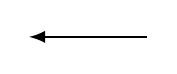
\begin{tikzpicture}[thick]
			\draw [black,   -latex, line width=1pt     ] (10.5,7.0) -- (9,7.0) node [right] {};
		\end{tikzpicture}
	\end{textblock*}	
	\begin{textblock*}{6cm}(7.5cm, 7.4cm)
		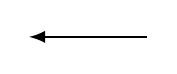
\begin{tikzpicture}[thick]
			\draw [black,   -latex, line width=1pt     ] (10.5,7.0) -- (9,7.0) node [right] {};
		\end{tikzpicture}
	\end{textblock*}	
	
	
	\begin{textblock*}{5cm}(9.2cm, 5cm)
		Champs de vitesse
	\end{textblock*}
	
	\begin{textblock*}{5cm}(9.2cm, 7.4cm)
		Dispersion
	\end{textblock*}

	
	
\end{frame}







\begin{frame}{Stages Master : M2 (IRAP)}
	\framesubtitle{Quelques résultats}
	\begin{columns}
		\begin{column}{0.5\linewidth}
			\vspace{-45pt}
			\begin{figure}
				\includegraphics[width=1.1\linewidth]{{graphics/SFR_sigma}.pdf}
			\end{figure}
		\end{column}
		\hfill
		\begin{column}{0.5\linewidth}
			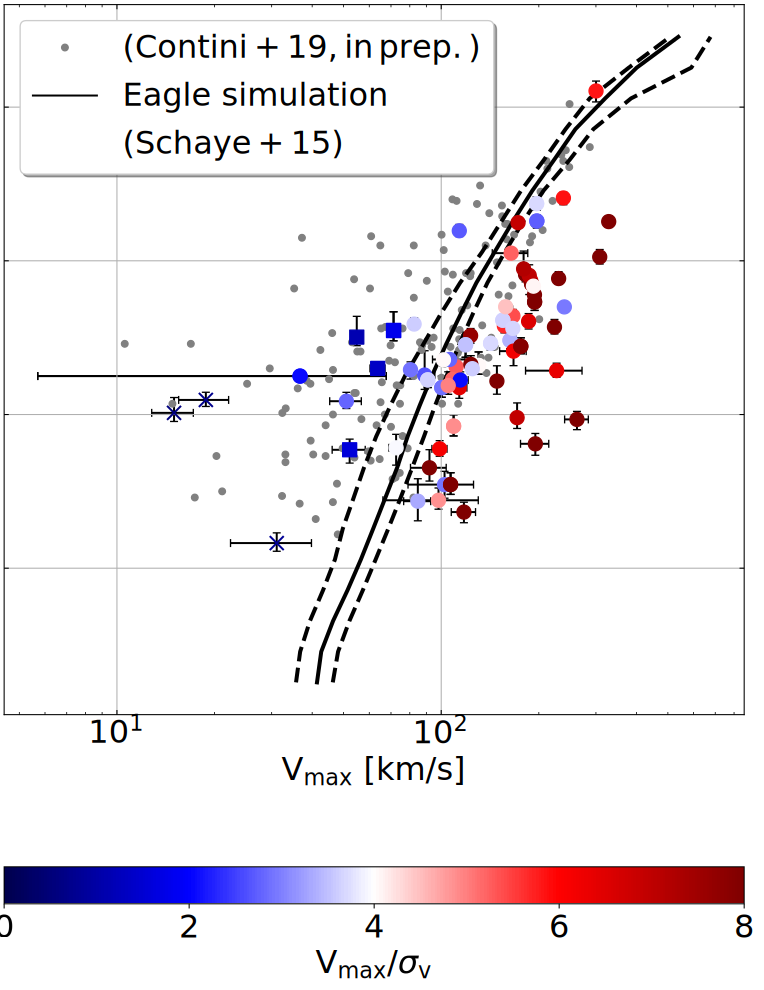
\includegraphics[width=0.9\linewidth]{{graphics/TFR_V_sigma}.eps}
		\end{column}
	\end{columns}
	\textbf{Relation $\mathbb{\rm{SFR} - \sigma_{\rm{v}}}$}  $\rightarrow$  à développer pendant la thèse.
	
	
	
	\begin{textblock*}{11cm}(4.8cm, 1.3cm)
		$\sim 100$ galaxies analysées
	\end{textblock*}
\end{frame}







\begin{frame}{Perspectives pour la thèse}

	\begin{textblock*}{6cm}(0cm, 1.5cm)
		\begin{itemize}[label=$\rhd$]
			\item Taille échantillon x10 \\(\textbf{+1000 galaxies}) !
		\end{itemize}
		\vfill			
		\begin{itemize}[label=$\rhd$]
			\item Impact de l'\textbf{environnement} aux petites (fusion, écoulement de gaz) et aux grandes échelles (groupes, amas) !
		\end{itemize}
		\vfill
		\begin{itemize}[label=$\rhd$]
			\item Nouvelles observations \textbf{ultra profondes} avec MUSE (150h)\\
				$\rightarrow$ Distribution de la \textbf{matière noire} très loin dans les galaxies
		\end{itemize}
			
		\begin{itemize}[label=$\rhd$]
			\item ELT + JWST\\
				$\rightarrow$ observation de galaxies "juste après" le Big Bang
		\end{itemize}
	\end{textblock*}
			
	
	\begin{textblock*}{5cm}(6cm, 1cm)
		\includegraphics[width=\linewidth]{{graphics/TF_groups_V_R22_sigma_scatter}.pdf}
	\end{textblock*}
	
	\begin{textblock*}{4cm}(8.8cm, 4cm)
		\includegraphics[width=\linewidth]{{graphics/Genzel2017}.png}
	\end{textblock*}
	
	\begin{textblock*}{6.5cm}(6.6cm, 1.3cm)
		\footnotesize\textbf{\textcolor{orange}{Abril-Melgajero+19, in prep.}}
	\end{textblock*}
	
	\begin{textblock*}{6.5cm}(9.4cm, 4.15cm)
		\footnotesize\textbf{\textcolor{orange}{Genzel et al. (2017)}}
	\end{textblock*}	
	
\end{frame}

\end{document}













